\documentclass[a4paper, 11pt]{article}
\usepackage{comment} % enables the use of multi-line comments (\ifx \fi) 
\usepackage{lipsum} %This package just generates Lorem Ipsum filler text. 
\usepackage{fullpage} % changes the margin

\usepackage[italian]{babel}
\selectlanguage{italian}
\usepackage[T1]{fontenc}
\usepackage[utf8]{inputenc}

\usepackage{graphicx}
\usepackage{hyperref}
\graphicspath{ {./images/} }

\begin{document}

%%%%%%%%%%%%%%%%%%%%%%%%%%%%%%%%%%%%%%%%%%%%%%%%%%%

\begin{titlepage}
	\centering
    \vspace*{0.5 cm}
    
\includegraphics[width=0.5 \linewidth]{images/ViceMediaLogo.png}\\[1.0 cm]
    \textsc{\LARGE Gestione Strategica delle Organizzazioni 18/19}\\[2.0 cm]
	\textsc{\Large Caso Unicorn}\\[0.5 cm]				
	\rule{\linewidth}{0.2 mm} \\[0.4 cm]
	{ \huge \bfseries Vice Media}\\
	\rule{\linewidth}{0.2 mm} \\[1.5 cm]
	
	\begin{minipage}{0.4\textwidth}
		\begin{flushleft} \large
			Giovanni Candeo\\
		\end{flushleft}
		\end{minipage}~
		\begin{minipage}{0.4\textwidth}
            
		\begin{flushright} \large
            Matricola N. 1206150\\
		\end{flushright}
        
	\end{minipage}\\[2 cm]
	
	
    
    
    
    
	
\end{titlepage}

%%%%%%%%%%%%%%%%%%%%%%%%%%%%%%%%%%%%%%%%%%%%%%

\newpage
\noindent
\begin{minipage}{0.3\textwidth}

\includegraphics[width=0.95 \linewidth]{images/ViceMediaLogo.png}
\end{minipage}
\hfill
\begin{minipage}{0.6\textwidth}\raggedleft
Azienda: Vice Media\\
Location: Brooklyn, New York, United States\\
Anno di costituzione: 1994 \\
Data di ingresso nella lista Unicorn: 8/17/2013 \\
Settore Principale: Digital Media \& News \\
\end{minipage}\\
\par\noindent\rule{\textwidth}{0.4pt}
\section*{Il problema da risolvere}
\par Gli ultimi 25 anni hanno mostrato un cambiamento radicale nel modo in cui le persone ottengono informazioni e "consumano" le notizie. Durante il ventesimo secolo i mezzi di comunicazione di massa si sono evoluti a partire dal giornale cartaceo, per passare alla radio e alla televisione. Ogni avvento di una nuova tecnologia ha reso la forma precedente per diffondere le notizie e i media sempre più obsoleta. Questo ha permesso di evidenziare un trend comune: le persone vogliono ottenere le informazioni e in particolar modo le notizie il più rapidamente possibile e sono disposte ad abbracciare qualsiasi nuova tecnologia che permette loro di farlo.\\
Internet e in particolare social media hanno la capacità di fornire le informazioni al pubblico in tempo reale con una disponibilità di ventiquattro ore al giorno per sette giorni alla settimana.\\
Con l’avvento di una nuova tecnologia nel mercato si aprono quindi nuovi problemi e domande da porsi: chi è disposto ad adottare questa “nuova” tecnologia e perché? Questa è una delle domande che si sono posti intorno al 2006 all’interno di Vice Media, decidendo di scommettere sui giovani.\\
Il problema da risolvere divenne quindi come riuscire a fornire una fonte di informazioni e notizie che si differenzia dai \textit{traditional media e  news} ma soprattutto \textit{appealing} per un pubblico giovane.

\section*{Concept di prodotto/servizio}
\par Originariamente l’azienda nasce come una rivista di musica punk per giovani chiamata \textit{Voice of Montreal} finanziata dal governo canadese attraverso fondi destinati allo sviluppo della musica, cultura e arte.
Ridenominata \textit{Vice} nel 1996, era vista come un alternativa alla concorrente \textit{Montreal Mirror}, la quale veniva però percepita troppo mainstream dalla fiorente sottocultura alternativa inglese della città, la cui linea di pensiero era rappresentata e riflessa nella crescita di collettivi come: \textit{Godspeed You! Black Emperor}, \textit{Dummies Theatre}, \textit{Bran Van 3000} e \textit{Arcade Fire} \cite{Mongaz}\cite{Mongaz2}. 
In comune con la rivista questi gruppi portavano la divulgazione e la celebrazione del multiculturalismo, della cultura punk e underground; ideali che si riflettono tutt’ora, seppur in minor modo, sullo stile dei contenuti di Vice Media e ritenuto da molti come aspetto fondamentale che contraddistingue l’azienda e causa principale del suo successo negli ultimi anni.\\
Vice Media attualmente si propone nel mercato come un azienda in grado di produrre contenuti multimediali a 360 gradi in controllo di vari business: multipli canali digitali di news, uno studio di produzione video e lungometraggi, un etichetta discografica, un’agenzia pubblicitaria interna, una pluripremiata serie-documentario su HBO e persino un pub a Londra; tutto questo conservando con cura la sua immagine “hipster” nell’industria dei media e dell’intrattenimento.

\newpage
\section*{Tecnologie adottate}
\par L'espansione precoce nel mondo digitale e di Internet è decisamente una delle cause principali del successo di Vice Media nel mercato dei digital media e news attuale.\\
Sebbene le tecnologie adottate dall'azienda (vedi tabella \ref{fig:tecnologie} in fondo) non è nulla di particolarmente innovativo, ciò che caratterizza sicuramente Vice Media è la costante espansione nel campo digitale. Questo infatti richiede l'adozione costante di tecnologie atte a permetterlo ed è riscontrabile nella storia dell'azienda tramite ad esempio gli accordi fatti con compagnie quali \textit{Rogers Communications} (comunicazione e broadcasting)  e \textit{Grupo Globo} (mobile).

\section*{Stima del mercato di riferimento (utenti primari)}
\par Il mercato in cui opera Vice Media è molto ampio dal momento che il focus dell'azienda sono i \textit{Digital Media} e l'intrattenimento. 
Questi comprendono infatti qualunque cosa che sia in formato digitale, come video, musica e articoli in formato digitale.\\
L'azienda in questione si focalizza principalmente sulle \textit{Digital News} in quanto i contenuti che produce sono finalizzati per la maggior parte a trattare temi d'attualità.

\subsection*{\textit{Dimensione del mercato e prospettive di crescita}}
\par Guidato dall’espansione dell’accesso a internet via mobile e dal continuo aumento della velocità di connessione, il numero crescente dei dispositivi mobili e di streaming sono la causa principale della crescita costante della domanda per ogni tipo di \textit{Digital Media} e nel particolare \textit{Digital News}, soprattutto a confronto dei mezzi tradizionali come quelli cartacei (vedi Figura \ref{fig:source}).\\ 
In modo particolare gli stati Asiatici dimostrano come un aumento di prosperità risulta in un desiderio esplosivo per la conoscenza, cultura e intrattenimento. In questo senso i media digitali di ogni tipo provvedono a soddisfare queste esigenze.\\
Confrontando i tre principali mercati di \textit{Digital Media}: gli Stati Uniti, la Cina e l’Europa; gli Stati Uniti sono il mercato più grande con un valore attuale di \$678 miliardi (vedi Figura \ref{fig:marketvalue}) contando un valore delle entrate di \$44.3 miliardi nel 2018.
Giudicando inoltre un alto valore di CAGR pari al 2.5\% le entrate nel mercato sono previste superare i \$50.2 miliardi nel 2023.\cite{Statista}


\subsection*{\textit{Segmentazione del mercato}}
\par Il mercato delle \textit{Digital News} all'interno dei \textit{Digital Media} si può segmentare per vari livelli: tipo di contenuto digitale, mezzi di distribuzione, topic o categoria del contenuto, area geografica, utente finale.\\
Vice spazia in tutto il mercato per quanto riguarda argomenti e tipo di contenuto, proponendo news in forma di articoli scritti sul proprio sito o anche video (documentari, brevi video, serie) per ogni tipo di piattaforma internet (ad accesso libero sui social media/youtube e in formato “subscription-based video-on-demand” su HBO) e non (tv via cavo con serie su canali quali MTV).
Vice si focalizza su un pubblico selezionato e ben preciso e non si sforza di essere una piattaforma in primo piano per quanto riguarda velocità e portata di distribuzione.\\
Per quanto riguarda il livello dell’area geografica, l’azienda è centrata principalmente in America ed Europa ma si sta espandendo sempre di più anche in Asia, Africa e Medio Oriente, contando al momento una presenza in più di 55 stati.

\subsection*{\textit{Concorrenza nel mercato}}
\par Segue l'analisi delle cinque forze di Porter (con riferimento a figura \ref{fig:porter}) per la posizione di mercato che occupa Vice Media:
\begin{itemize}
\item  Minaccia di nuovi entranti: \textit{Media} - Nonostante la possibilità di creare contenuti online al giorno d’oggi sia a portata di tutti, la creazione di una fonte di notizie e contenuti digitali di qualità pari a quella che portano nel mercato Vice Media e i suoi \textit{competitors} è tutt’altro che semplice.  A maggior ragione se andiamo ad osservare la fetta di mercato specifico che sono i giovani e in particolare i “millennials”.
\item Minaccia di prodotti e servizi sostitutivi: \textit{Alta} – Come già scritto in precedenza, il mercato delle News e dei Digital Media è caratterizzato da un continuo susseguirsi di nuovi prodotti tecnologici adottati dal pubblico che rende indispensabile la costante attenzione nel mercato da parte delle aziende nel settore.
\item Potere contrattuale dei fornitori: \textit{Alto} – Nel mercato dei media e delle News in particolare il potere contrattuale dei fornitori è alto; degli esempi possono essere qualunque tipo di evento o contenuto esclusivo  che l’azienda deve portare sulla propria piattaforma per fare concorrenza alle aziende rivali.
\item Potere contrattuale dei clienti: \textit{Molto alto} – In questo mercato in particolare ci sono due tipi di clienti principali: il pubblico e inserzionisti. Gli inserzionisti sono i principali clienti per i Digital Media e soprattutto le \textit{Online News}. In questo segmento di mercato infatti c’è una sproporzione fra la domanda e l’offerta: i clienti hanno il potere di scegliere tra più piattaforme su cui piazzare la propria pubblicità e ciò spinge i prezzi e i margini a vantaggio degli inserzionisti. A tal proposito ritengo noto menzionare che Vice ha rischiato più volte di mettere a rischio il suo brand e la sua immagine pur di soddisfare gli obblighi contrattuali con i propri sponsor e clienti.
\item Rivalità tra le imprese esistenti: \textit{Alta} – Come risultato delle quattro forze analizzate qui sopra si può notare uno scenario di alta rivalità e competizione tra gli operatori in questo mercato.
\end{itemize}

\section*{Profilo dell’utente primario e degli altri (potenziali) utenti}
\par Vice seleziona un audience molto specifico per i suoi contenuti: persone giovani nella fascia d'eta 18-30 anni che vogliono notizie approfondite e incisive presentate in un modo coinvolgente.
Ciò che interessa all'audience di Vice non è la rapidità con cui vengono presentate le notizie ma il modo in cui vengono raccontate.\\
Dopo l'ormai affermato successo sul web, l'azienda ha cercato di conquistare sempre di più anche il mondo dei \textit{traditional media} attraverso show televisivi e quello del cinema attraverso documentari e lungometraggi come \textit{"Fishing Without Nets"} e\textit{ "The Bad Batch"} riconosciuti da grandi festival cinematografici statunitensi e internazionali.

\newpage
\section*{Analisi dei competitor e differenziazione}
\par Il competitor principale di Vice è \textit{Buzzfeed}.\\ 
\textit{Buzzfeed} è un'azienda ormai diffusa globalmente di notizie e intrattenimento sociale che produce e distribuisce notizie originali, intrattenimento e video.
La differenza principale tra Vice e Buzzfeed è decisamente la differenza nel tipo di contenuto: Buzzfeed preferisce focalizzarsi su contenuto virale e più "leggero" rispetto a Vice Media che preferisce invece trattare invece temi più maturi e soprattutto controversi.\\
Un esempio lampante lampante di questa differenza tra i due brand si può notare visitando le pagine web principali delle due aziende: mentre Buzzfeed presenta argomenti etichettati sotto categorie quali "Animali", "Cibo", "Viaggi", Vice presenta invece temi quali "Politica", "Cultura", "Droga" e "LGBTQ".\\
Indicativo per la differenziazione dell'azienda è anche la figura \ref{fig:difference}, che mostra il focus principale dell'azienda in: contenuti per un pubblico giovane, giornalismo immersivo e contenuti da "dietro le quinte" approfonditi. 


\section*{Modello di business e fonti di ricavo}
\textit{“What we really have at the end of the day is our brand, and if we screw that up we have nothing… We don’t want to be sellouts”} - Eddy Moretti, Chief Creative Officer nel 2014\\

\par Il modello di business di Vice è molto simile a quello delle aziende tradizionali nel campo media dove la pubblicità è la fonte principale di profitto.
La differenza principale tra i media tradizionali e Vice è che quest’ultima ha abbracciato molto prima il mondo di Internet, sia dal punto di vista del contenuto che dal punto di vista di modello pubblicitario, riuscendo quindi a crearsi una rete di utenti prima della concorrenza e quindi il vantaggio competitivo.
Il modello di business di Vice punta molto sul proprio brand e sulla sua immagine sul mercato, puntando ad attrarre un pubblico specifico, i giovani, e identificando il modo migliore per diffondere il proprio contenuto  adottando anche un innovativo sistema di pubblicità.\\
Un strategia che Vice ha adottato e che riflette questo è ad esempio il mantenimento della presenza su HBO, atta a stabilire una maggiore connessione con il pubblico più giovane che associa la piattaforma a show popolari come \textit{Games of Thrones}.


\section*{Profilo dei Founders}
\subsection*{\textit{Suroosh Alvi}}
Suroosh Alvi nasce nel 1969 a Toronto da genitori pakistani, entrambi professori univeritari; il padre è professore in psicologia, la madre in studi islamici e storia di Mughal.
Alvi studia filosofia alla \textit{MgGill University} in Montreal, città in cui lancia VICE nel 1994 insieme a Shane Smith e Gavin McInnes.\\
Nel 2006 Suroosh pubblica un segmento sul mercato delle armi in Pakistan che ebbe particolarmente successo e da allora ha iniziato a coprire storie di altri parti del mondo quali: Repubblica Democratica del Congo, Pakistan, Afghanistan e la Striscia di Gaza.\\
In seguito ha prodotto e condotto documentari Vice su HBO, \textit{VICE News} e la serie \textit{VICE Travel}.\\
Nel 2017 ha lanciato una serie in più parti esaminando le origini e l'impatto delle organizzazioni terroristiche più letali del mondo: al Qaeda nello Yemen, al Shabaabin in Somalia, Boko Haram in Nigeria, Tehrik-i-Taliban in Pakistan e Stato Islamico in Iraq.

\subsection*{\textit{Shane Smith}}
Shane Smith nasce ad Ottawa nel 1969 e si laurea alla \textit{Carleton University} in letteratura inglese e scienze politiche.
Prima di trasferirsi a Montreal e fondare VICE nel 1994, Shane suona in vari gruppi punk locali e fa viaggi in Est Europa.
Come giornalista, Smith ha viaggiato in luoghi come la Corea del Nord, l'Iran, l'Afghanistan, il Kashmir, la Liberia e la Groenlandia principalmente per la serie TV online del 2006 \textit{VICE Guide to Travel}.\\
Attualmente è presidente esecutivo di Vice Media.

\subsection*{\textit{Gavin McInnes}}
McInnes è nato nel 1970 a Hitchin in Hertfordshire, in Inghilterra, da genitori scozzesi. La sua famiglia migrò in canada nel 1974 e da adolescente ha suonato in gruppi punk locali di Ottawa.\\
Co-fondatore di Vice nel 1994 è stato descritto come il “padrino della cultura Hipster” dalla WNBC. 
Lascia la compagnia nel 2008 a causa delle “differenze creative” con l’azienda e il suo avvicinamento politico all’estrema destra.

\section*{Investimenti ottenuti}
\par Gli investimenti ottenuti dall’azienda riportati nella tabella in figura \ref{fig:investimenti} sono importanti in quanto indicano i segni di fiducia del mercato nel potenziale di Vice Media. La \textit{Twenty-First Century Fox} ha investito 70 milioni di dollari per una quota del 5\% di Vice nel 2013, valutando la società a \$ 1.4 miliardi.
\textit{A\&E} ha pagato a \$ 250 milioni per una partecipazioni del 10\% nella società nel 2014.
\textit{Disney} ha investito \$ 400 milioni in Vice nel 2015, valutando la società a \$ 4.5 miliardi.\\
Ciò che attrae principalmente questi investimenti è la capacità di Vice di generare reddito tramite inserzioni pubblicitarie nelle sue piattaforme, a differenza dei media tradizionali.
Questi investimenti sono anche indicativi della potenza del mercato dei \textit{millennial}.\\
Tramite questi investimenti Vice sarà in grado di ampliare le proprie offerte per competere con i concorrenti, questo soprattutto tramite lo sviluppo di più documentari e lungometraggi che la differenzia dal principale competitor Buzzfeed, il cui successo è riconosciuto a contenuto più corto e progettato per una diffusione virale.

\section*{Prospettive future dell’impresa}
Vice Media è riuscita ad affermarsi in un settore del mercato molto competitivo grazie al suo marchio portabandiera della contro-cultura e dell'anticonformismo. La sua recente espansione globale e i sempre più frequenti accordi con società \textit{mainstream} rischiano di far perdere l'autenticità del brand, che è stato ed è chiave del successo del modello di business dell'azienda.\\
A causa dei molteplici contratti di sponsorizzazione e il modello di pubblicità dei contenuti proposti, Vice Media è stata criticata più volte in passato per vendere pubblicità alle grandi società e soprattutto rendere meno evidenti i confini tra il contenuto editoriale e pubblicitario \cite{gawker}.
Nel 2017, Vice ha dichiarato di aver perso \$ 100 milioni ed è prevista la perdita di altri \$ 50 milioni per il 2018, nonostante sia in grado di vantare una valutazione di \$ 5,7 miliardi, la più alta di qualsiasi nuova azienda nel settore dei media\cite{glenday}.\\
La domanda è quindi: riuscirà Vice Media a continuare la sua espansione nel mondo digitale delle news e dell'intrattenimento mantenendo l'autenticità del proprio brand?\\



\newpage
\section*{Figure}
\null
\vfill
\begin{figure}[h]
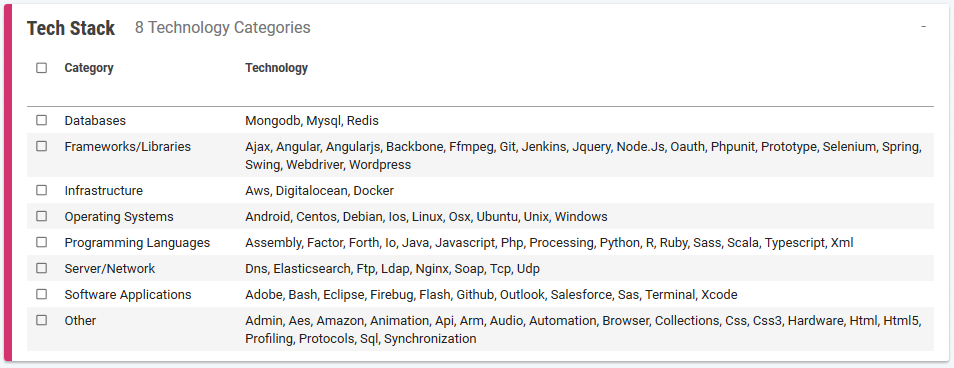
\includegraphics[width=\textwidth]{images/viceTech.PNG}
\caption{Tabella delle tecnologie adottate.}
\label{fig:tecnologie}
\end{figure}
\begin{figure}[h]
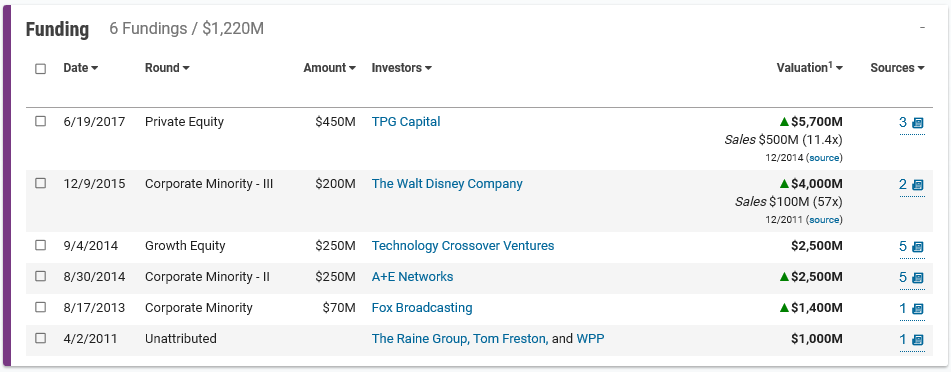
\includegraphics[width=\textwidth]{images/viceFundings.PNG}
\caption{Tabella dei finanziamenti ottenuti}
\label{fig:investimenti}
\end{figure}
\vfill

\newpage\null\vfill
\begin{figure}[h]
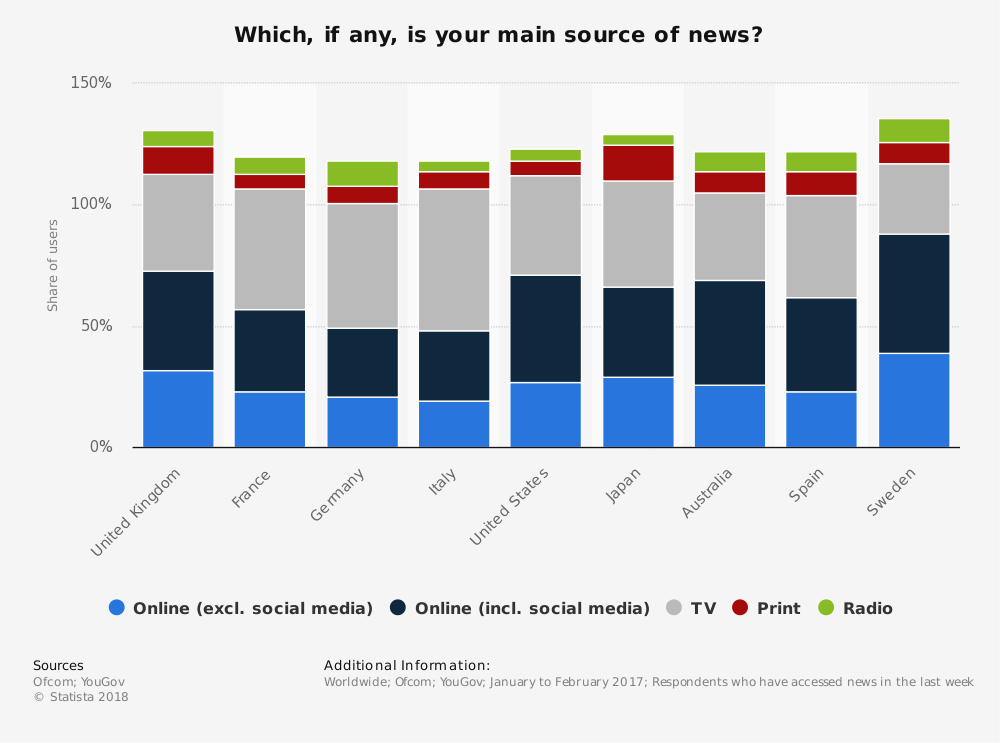
\includegraphics[width=\textwidth]{images/vicenewssource.png}
\caption{Fonti di reperimento delle news per area geografica.}
\label{fig:source}
\end{figure}
\vfill

\newpage\null\vfill
\begin{figure}[h]
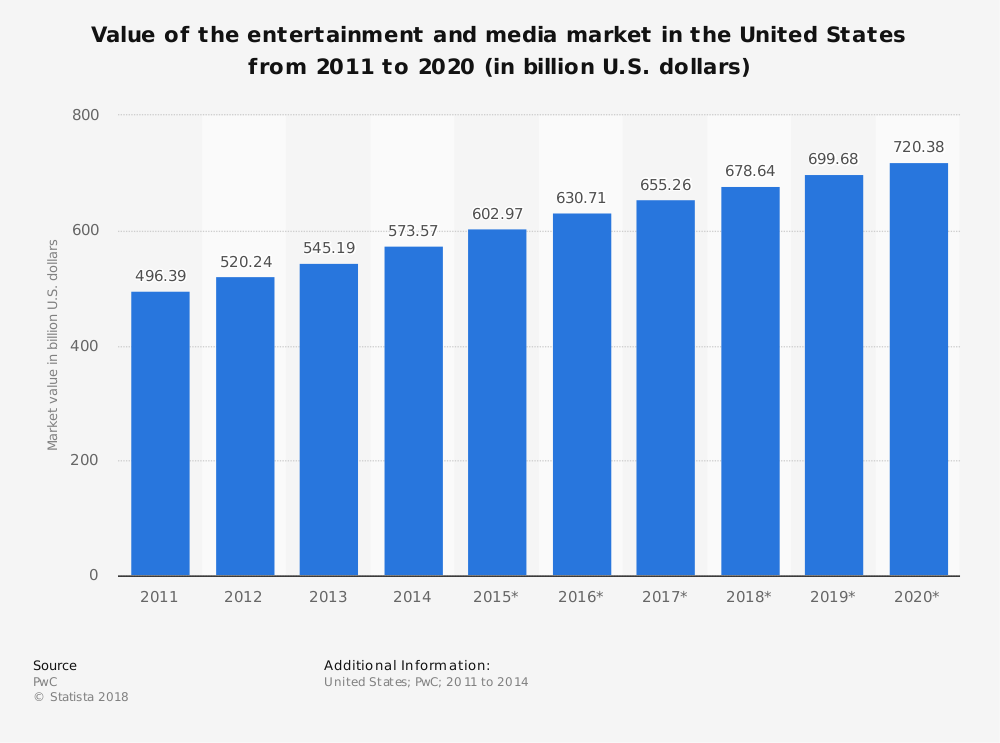
\includegraphics[width=\textwidth]{images/vicemarketvalue.png}
\caption{Valore del mercato statunitense dei media e dell'intrattenimento.}
\label{fig:marketvalue}
\end{figure}
\vfill

\newpage\null\vfill
\begin{figure}[h]
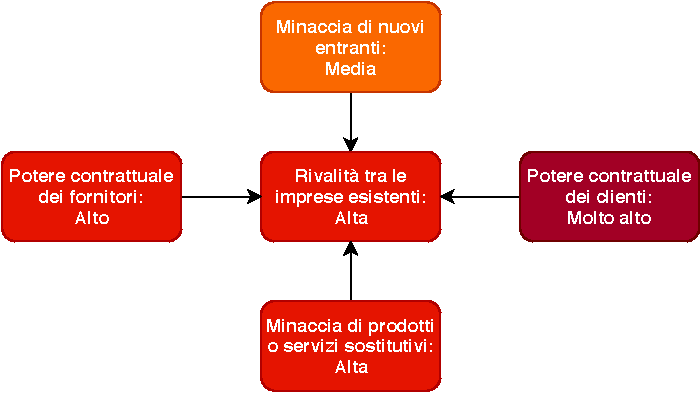
\includegraphics[width=\textwidth]{images/porter.pdf}
\caption{Modello delle cinque forze competitive di Porter per il mercato dei Digital Media e News.}
\label{fig:porter}
\end{figure}
\vfill

\newpage\null\vfill
\begin{figure}[h]
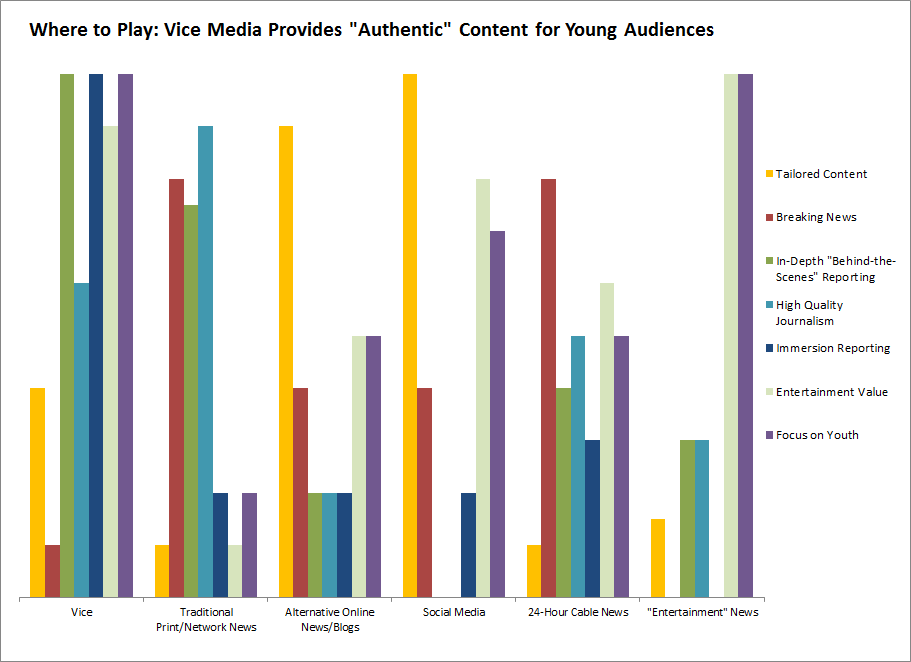
\includegraphics[width=\textwidth]{images/vicepositioning.png}
\caption{Differenziazione dei contenuti di Vice Media.\cite{forsan}}
\label{fig:difference}
\end{figure}
\vfill

\newpage
\section*{Note}
Informazioni principali dell'azienda ottenute grazie anche a \href{www.wikipedia.org}{Wikipedia}.\\
Aziende \textit{competitor} ottenute dal profilo dell'azienda su \href{www.cbinsights.com}{\textit{CB Insights}}.\\
Tabella delle tecnologie adottate ottenute dal profilo dell'azienda su \href{www.cbinsights.com}{\textit{CB Insights}}.\\
Grafici in figura \ref{fig:source} e \ref{fig:marketvalue} ottenuti su Statista.com [www.statista.com].\\
Il codice sorgente LaTeX utilizzato per creare questo report è disponibile nella repository GitHub. [https://github.com/candeogi/HomeworkGSO].\\

\begin{thebibliography}{9}
\bibitem{Statista} \emph{"Digital Media Report 2019"}. Statista. Dicembre 2018.
\bibitem{Mongaz} Kelly, Brendan. \textit{Vice...and alternative anglos}. Montreal Gazzette, 26 Marzo 2014.
\bibitem{Mongaz2} Kelly, Brendan. \textit{Quebec culture, the solitudes and the theatre of the absurd}, Montreal Gazzette, 22 Marzo 2014.
\bibitem{forsan} Joseph Bateman, Aditi Manocha, Elizabeth Peyton,
Alexander Soley, Alexandra Taylor. \textit{The journey so far and the road ahead}. Aprile 2015. 
\bibitem{gawker} Nolan, Hamilton. \textit{The Revolution Will Not Be Vice}. Gawker, 19 Agosto 2013. 
\bibitem{glenday} Glenday, John. \textit{Vice Media to reduce workforce by 15\% and consolidate digital brands as growth stalls}. The Drum, 8 Novembre 2018.

\end{thebibliography}

\end{document}
